\subsection{Concepts in Manifold Learning}
\label{mani-concepts}

This chapter introduces the main geometric concepts considered necessary to
provide a solid understanding of SS-LLE\footnote{
Obviously, the list of concepts discussed is by no means extensive. Theory is
presented much more in detail (and mathematical rigor) in, for example, 
% FIXME Put in source
\textcolor{red}{good book}.
}.
It must be noted that everything discussed here is presented through the lens of
machine learning, deliberately forsaking the generality inherent to topology.
Therefore, assuming features can be represented by coordinates in 
$D$-dimensional Euclidean space, all concepts are examined with regard to their
meaning in $\RD$.
Dimensionality reduction techniques take the data observed in $\RD$ to actually
lie on a $d$-dimensional topological space that is not necessarily Euclidean but
exhibits some specific properties.
\\

% FIXME Make enumeration more compact 

\textbf{Topological spaces.} A \textit{topological space} is constituted by a 
set $T$ equipped with a \textit{topology} $\topo$. 
A topology is a general way of describing relations between elements in $T$.
Consider a function $\topo: T \rightarrow 2^T, t \mapsto \topo(t)$, which 
assigns to $t \in T$ a set of subsets of $T$ called \textit{neighborhoods}.
For $\topo$ to be a topology\footnote{
Alternative definitions employ open subsets of $T$, see for example 
\citet{waldmann2014}.
}
on $T$, the following properties must hold \citep{brown2006}:
\begin{tight_enumerate}
  \item If $\topo$ is a neighborhood of $t$, then $t \in \topo$.
  \item If $\topo$ is a subset of $T$ containing a neighborhood of $t$, then 
  $\topo$ is a neighborhood of $t$.
  \item The intersection of two neighborhoods of $t$ is again a neighborhood of
  $t$.
  \item Any neighborhood $\topo$ of $t$ contains a neighborhood $\topo^{\prime}$ 
  of $t$ such that $\topo$ is a neighborhood of each element in 
  $\topo^{\prime}$.
\end{tight_enumerate}

Note that, in this general definition, neighborhoods are based on an abstract
notion of "nearness". 
Learning the structure of a topological space effectively boils down to learning 
neighborhood relations.
In Euclidean topological space these are directly based on distance: 
neighborhoods around $t$ are constructed by $\epsilon$-balls containing all 
elements within a Euclidean distance of $\epsilon$ from $t$. 
The resulting topology is also called the \textit{metric topology} 
\citep{mccleary2006}.

Topological spaces in general are not accessible via distances (or angles, for 
that matter) known from Euclidean spaces.
The ultimate goal therefore is the interpretation of the data in a space that is 
again Euclidean, albeit of lower dimensionality, where such concepts are 
meaningful.
The next step is then to study how (potentially highly non-linear) topological 
spaces relate to $\Rd$.
\\

\textbf{Homeomorphisms.} Consider two topological spaces $(S, \topo_S)$, 
$(T, \topo_T)$ (denoted by the respective shorthands $S$, $T$ from here) and a 
mapping function $f: S \rightarrow T$. 
If $f$ is bijective and continuous and $f^{-^1}: T \rightarrow S$ is also 
continuous, $f$ is called a \textit{homeomorphism} \citep{brown2006}.
Topological spaces for which such a mapping exists are \textit{homeomorphic} to
each other. 
Any properties of $S$ that $T$ shares when it is homeomorphic to $S$ are 
referred to as topological properties. 
Two homeomorphic spaces are thus topologically equivalent \citep{mccleary2006}.

If there exists a non-negative integer $d$ such that for every $s$ in a 
topological space $S$ a local neighborhood $U \ni s$, $U \subset S$, is 
homeomorphic to an open subset of $\Rd$ (sometimes called \textit{parameter 
space}), $S$ is \textit{locally 
Euclidean}\footnote{
For locally Euclidean topological spaces it is thus meaningful to speak of
elements as points.
} \citep{mafu2011}.
In other words, there is a homeomorphism $f: U \rightarrow \Rd$ for every 
element in $S$.
The neighborhoods $U$ are also referred to as  \textit{coordinate patches} and 
the associated maps $f$ are called \textit{coordinate charts} 
\citep{cayton2005}.
In local neighborhoods $S$ then behaves like $\Rd$ \citep{mafu2011}.
\\

\textbf{Manifolds.} \textit{Manifolds} are now precisely such locally Euclidean
topological spaces, with some additional properties.
For a topological space $\mani$ to be a $d$-dimensional manifold\footnote{
$\mani$ is again a shorthand, omitting the explicit notation of the 
corresponding topology. 
} (also: $d$-manifold) it must meet 
the following conditions \citep{waldmann2014}:

\begin{tight_enumerate}
  \item $\mani$ is Hausdorff.
  \item $\mani$ is second-countable.
  \item $\mani$ is locally homeomorphic to $\Rd$.
\end{tight_enumerate}

The Hausdorff condition is a separation property and ensures that for any two 
distinct points from $\mani$ disjoint neighborhoods can be found 
\citep{brown2006}.
Second-countability restricts the manifold's size via the number of open sets 
it may possess \citep{waldmann2014}.
\\

\vspace{0.5cm}

% TODO Mark 2 points on S-curve and connect via Euclidean distance

\begin{minipage}[b]{0.5\textwidth}
  \textbf{Embeddings.} Recall that the data are observed in $\RD$ but taken to 
  lie on $\mani$, locally homeomorphic to $\Rd$.
  This implies the assumption $\mani \subset \RD$ and $\mani$ is said to be 
  \textit{embedded} in the ambient $D$-dimensional Euclidean space 
  \citep{cayton2005}.
  The associated \textit{embedding} is but a map $f: \mani \rightarrow \RD$ 
  whose restriction to $\mani$ is a homeomorphism \citep{brown2006}, or, more 
  specifically, the canonical inclusion map identifying points on the manifold 
  as particular points of $\RD$ \citep{waldmann2014}.
  It can be shown that $K = 2d + 1$ is sufficient to create an embedding 
  \citep{mafu2011}.
  Figure \ref{fig:scurve} shows the so-called \textit{S-curve} manifold 
  embedded in $\R^3$.
  Clearly, the S-curve as a whole is far from linear, but locally homeomorphic 
  to $\R^2$ and thus intrinsically two-dimensional.
\end{minipage}
\begin{minipage}[b]{0.05\textwidth}
  \phantom{xxx}
\end{minipage}
\begin{minipage}[b]{0.45\textwidth}
  \begin{figure}[H]
    \centering
    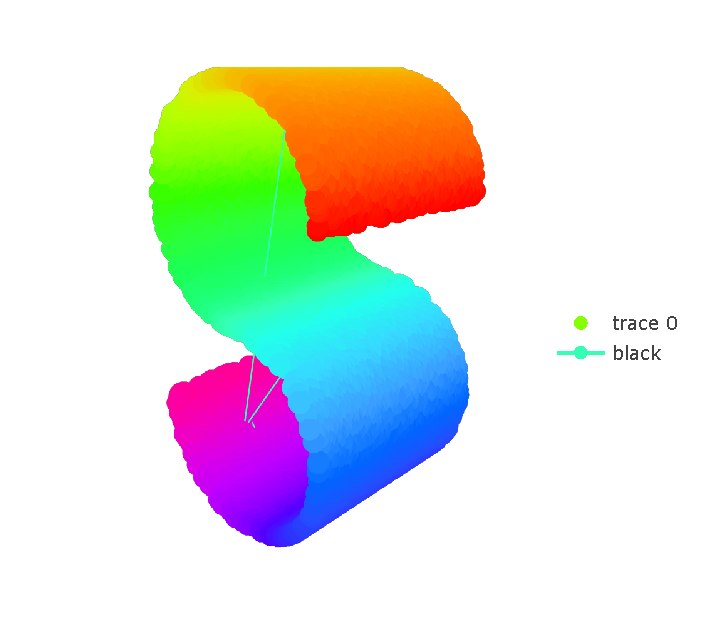
\includegraphics[trim = 100 20 70 30, clip, % left bottom right top
      width = 0.65\textwidth]{figures/s-curve}
    \caption[S-curve manifold]{10,000 points sampled from the S-curve manifold. 
    \textit{Source:} own representation, inspired by implementation in 
    \texttt{Python}'s \texttt{scikit-learn} library \citep{scikit-learn}.}
    \label{fig:scurve}
  \end{figure}
\end{minipage}

\vspace{0.5cm}

\textbf{Geodesics.} One last aspect remains open and shall be briefly touched 
here, namely how to handle distances on manifolds where Euclidean metrics are 
not meaningful.
Rather than measuring "shortcuts" between points across $\RD$ (where, for 
instance, points in the red upper area of figure \ref{fig:scurve} would be 
considered deceptively close to points in the cyan mid area), it makes intuitive 
sense to constrain distances to the manifold surface.
In order to enable the construction of such a metric, manifolds must fulfill
two additional properties: \textit{smoothness}\footnote{
The smoothness property is based on differentiability of coordinate charts and 
ensures that concepts of curvature, length and angle remain meaningful 
\citep{mafu2011}.
A detailed derivation may be found, for example, in \citet{mukherjee2015}.
} and \textit{connectedness}\footnote{
Connectedness means that no separation $\{ U, V\}$ of a manifold 
$\mani$ exists with open, non-empty and disjoint $U, V \subset \mani$, 
$\mani = U \cup V$.
This may be loosely put as paths linking arbitrary pairs of manifold points 
\citep{mccleary2006}.
} \citep{mafu2011}.
For smooth, connected manifolds, \textit{geodesic distance} is the length of the 
shortest curve (\textit{geodesic}) on $\mani$ between two points on $\mani$.
A curve $c$ in $\mani$ is a smooth mapping from an open interval $\Lambda 
\subset \R$ into $\mani$.
$c$ is parametrized by a point $\lambda \in \Lambda$, such that
$c(\lambda) = (c_1(\lambda), ..., c_d(\lambda))^T$ (all $c_j, j = 1, ..., d$,
having a sufficient number of continuous derivatives) is a curve in $\Rd$.
Component-wise differentiation with respect to $\lambda$ yields the
\textit{velocity} of $c$ in $\lambda$, $c^{\prime}(\lambda) =
(c_1^{\prime}(\lambda), ..., c_d^{\prime}(\lambda))^T$.
The \textit{speed} of $c$ is given by $\| c^{\prime}(\lambda) \|^2_2$, where
$\| \cdot \|^2$ denotes the square norm.
Then, distance along this curve is measured by the arc-length
$L(c) = \int_{\pv}^{\qv} \| c^{\prime}(\lambda) \|^2 d\lambda$.
Finally, geodesic distance can be derived as the length of the shortest such
curve, out of the set of differentiable curves in $\mani$ that connect $\pv$ and
$\qv$, $\mathcal{C}(\pv, \qv)$: \\
$d^{\mani}(\pv, \qv) = \inf_{c \in \mathcal{C}(\pv, \qv)} L(c)$
\citep{mafu2011}.
Intuitively, geodesic distance can be identified with Euclidean distance in
Euclidean spaces where shortest curves are just straight lines \citep{mafu2011}.

% as 
% measured by arc-length\footnote{
% Geodesics are but a peripheral note here; for a precise definition see 
% \citet{mafu2011}.
% }.






% ------------------------------------------------------------------------------

\subsection{Formal Goal of Manifold Learning}
\label{mani-goal}

Building on the above concepts, the data situation in manifold learning 
might be summarized as follows: data are observed in $\RD$ but assumed to 
be really samples from a $d$-manifold $\mani$ embedded in $\RD$, meaning they 
can be analyzed in $\Rd$ if a faithful translation between respective 
coordinates in $\RD$ and $\Rd$ is found\footnote{
It is actually a simplification to assume all data to lie \textit{exactly} on 
$\mani$, but the more general case of data lying \textit{near} $\mani$ is rarely 
considered explicitly.
}.
The challenge is thus to unravel the manifold in a way that preserves its 
intrinsic structure to maximum extent \citep{sauletal2006}.
This goal shall be formalized in a way that will be referenced throughout the 
remainder of this report and that is inspired by the works of \citet{cayton2005} 
and \citet{sauletal2006}.
\\

\textbf{Given.} Data $\X = (\x_1, \x_2, ..., \x_N)$, with 
$\x_i \in \RD$ $\forall i \in \setN$ and $N, D \in \N$. 
$\X$ thus consists of $N$ real-valued data vectors observed in $D$ 
dimensions.
The true data-generating process is taken to have dimensionality $d \in \N$, 
such that $\X$ is in fact a sample from a smooth, connected $d$-manifold with
$\X \sim \mani \subset \RD$.
$\mani$ may be described by a single coordinate chart\footnote{
This is possible for any smooth, compact manifold \citep{cayton2005}.
} $\psi: \mani \rightarrow \Rd$.
For manifold learning methods to yield satisfying results, $\mani$ is always 
assumed to be sampled well by $\X$.
\\

\textbf{Goal.} Find the $d$-dimensional representation of the data, 
i.e., compute \\$\Y = (\y_1, \y_2, ..., \y_N)$, where 
$\y_i = \psi(\x_i) \in \R^d$ $\forall i \in \setN$.
The map $\psi$ itself is not always explicitly retrieved.
\\

Note that, while $D$ is given a priori, the intrinsic dimensionality $d$ is 
often unknown in real-life applications.
Due to the lack of (finite-sample) convergence guarantees for many methods 
dimensionality estimations may not always be equal to $d$.
$\Y$ as found by manifold learning techniques must therefore be expected to 
differ from the true coordinates and, in particular, to even have incorrect 
dimension \citep{sauletal2006}.
Notwithstanding this potential gap, solutions of the subsequently presented 
methods will be denoted by $\Y \in (\Rd)^N$ to avoid overly complicated 
notation.
